\subsubsection{Interfaces}
zum einschalten der Interfaces habe ich im conf terminal des Routers einfachen die folgenden Befehle eingegeben:
\begin{lstlisting}
Router(config)#int range gig0/0-2
Router(config-if-range)#no shutdown
Router(config-if-range)#end
\end{lstlisting}
\begin{figure}[!htb]
    \centering
    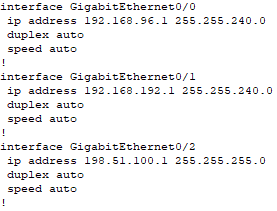
\includegraphics[width=\textwidth,height=.35\textwidth,keepaspectratio]{./img/config/interfaces.png}
    \caption{Running Config des Routers}
\end{figure}
\begin{figure}[!htb]
    \centering
    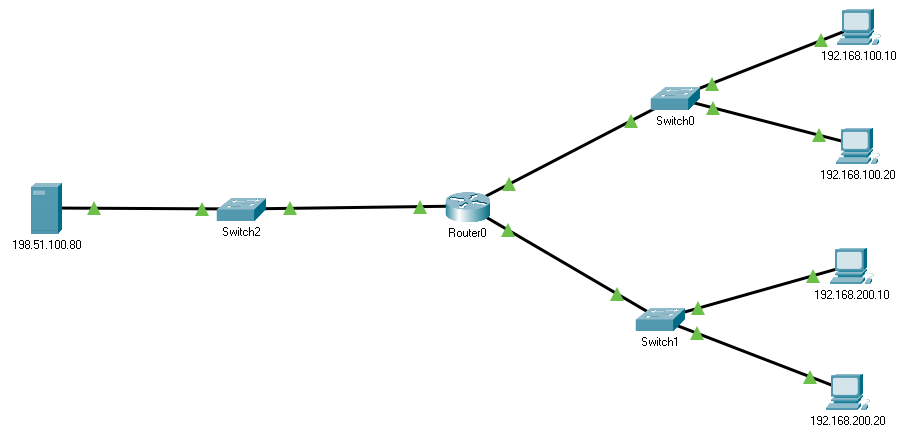
\includegraphics[width=\textwidth,height=.6\textwidth,keepaspectratio]{./img/config/end.png}
    \caption{Konfiguration nach einschalten des Routers}
\end{figure}
\FloatBarrier

\subsubsection{Frage 1}
\paragraph{Frage}
Wie kann die niedrigste freie Adresse in einem Netz errechnet werden,
und welche Adressen sind das in den gegebenen Netzen?
\paragraph{Antwort}
Man berechnet die Subnet Id zuerst. Dies wird ermöglicht in dem man die Netzmaske und die IP Adresse mit einem binären UND rechnet. Das Ergebnis wird um 1 erhöht und das ist die Adresse.\\
Die Berechnungen habe ich mit einem selbstgeschriebenem TS Programm durchgeführt.\\
Das Programm befindet sich zur Sicherheit im zip folder.\\
192.168.100.x/20 = 192.168.96.1 \\
192.168.200.x/20 = 192.168.192.1 \\
198.51.100.x/24 = 198.51.100.1
\begin{figure}[!htb]
    \centering
    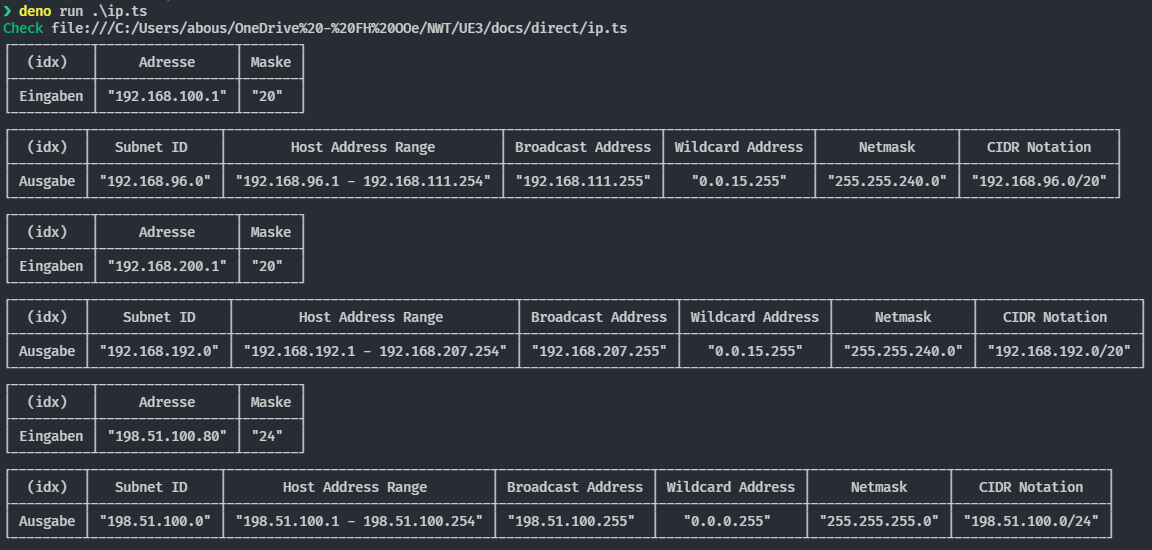
\includegraphics[width=\textwidth]{./img/config/frage1.png}
    \caption{Resultate der Berechnungen}
\end{figure}
\subsubsection{IPv6}
\subsubsection{Endsysteme}
\subsubsection{Frage 2}

